\section{项目背景与任务描述}
\label{sec:background}
\subsection{从视觉语言技术到膳食记录}
随着深度学习和视觉语言模型的发展，图像描述生成技术能够将视觉信息转化为自然语言，在智能图像理解、辅助信息获取和内容检索等领域具有应用价值。从 CNN 与循环网络组成的编解码模型，到引入空间注意力和多模态预训练的生成模型，研究逐步从识别图像中的对象，拓展到描述对象的属性、关系与场景\cite{vinyals2015show,xu2015attend,bai2025qwen}。食物图像是其中具有代表性的细粒度场景：一张餐照中既有整道菜的外观，也有分散、遮挡或混合在一起的配料，仅给出菜品类别难以完整表达其内容。

以食堂用餐为例，照片可以保留餐盘当时的模样，却不便直接检索“哪些餐有水果”或汇总不同餐次的组成。自然语言描述可以将可见食物、颜色与形态转成便于回顾的文字；结构化记录则进一步把食材名称、重量及整餐营养组织为统一字段，支持程序检索和逐项核对。图~\ref{fig:meal-evidence}展示了从餐食照片到这两类记录的任务关系。FoodLens 因此以单张 RGB 图像为输入，研究食物描述生成与结构化膳食记录生成，并检验语义识别、数值估计和输出格式之间的联系。

\begin{figure}[!ht]
\centering
% Editable task illustration. Examples are manually written, not predictions.
\begin{tikzpicture}[x=1cm,y=1cm]
\node[fllabel,anchor=west] at (0,2.7) {输入：单张餐食 RGB 图像};
\node[inner sep=0] (meal) at (2.35,.1)
 {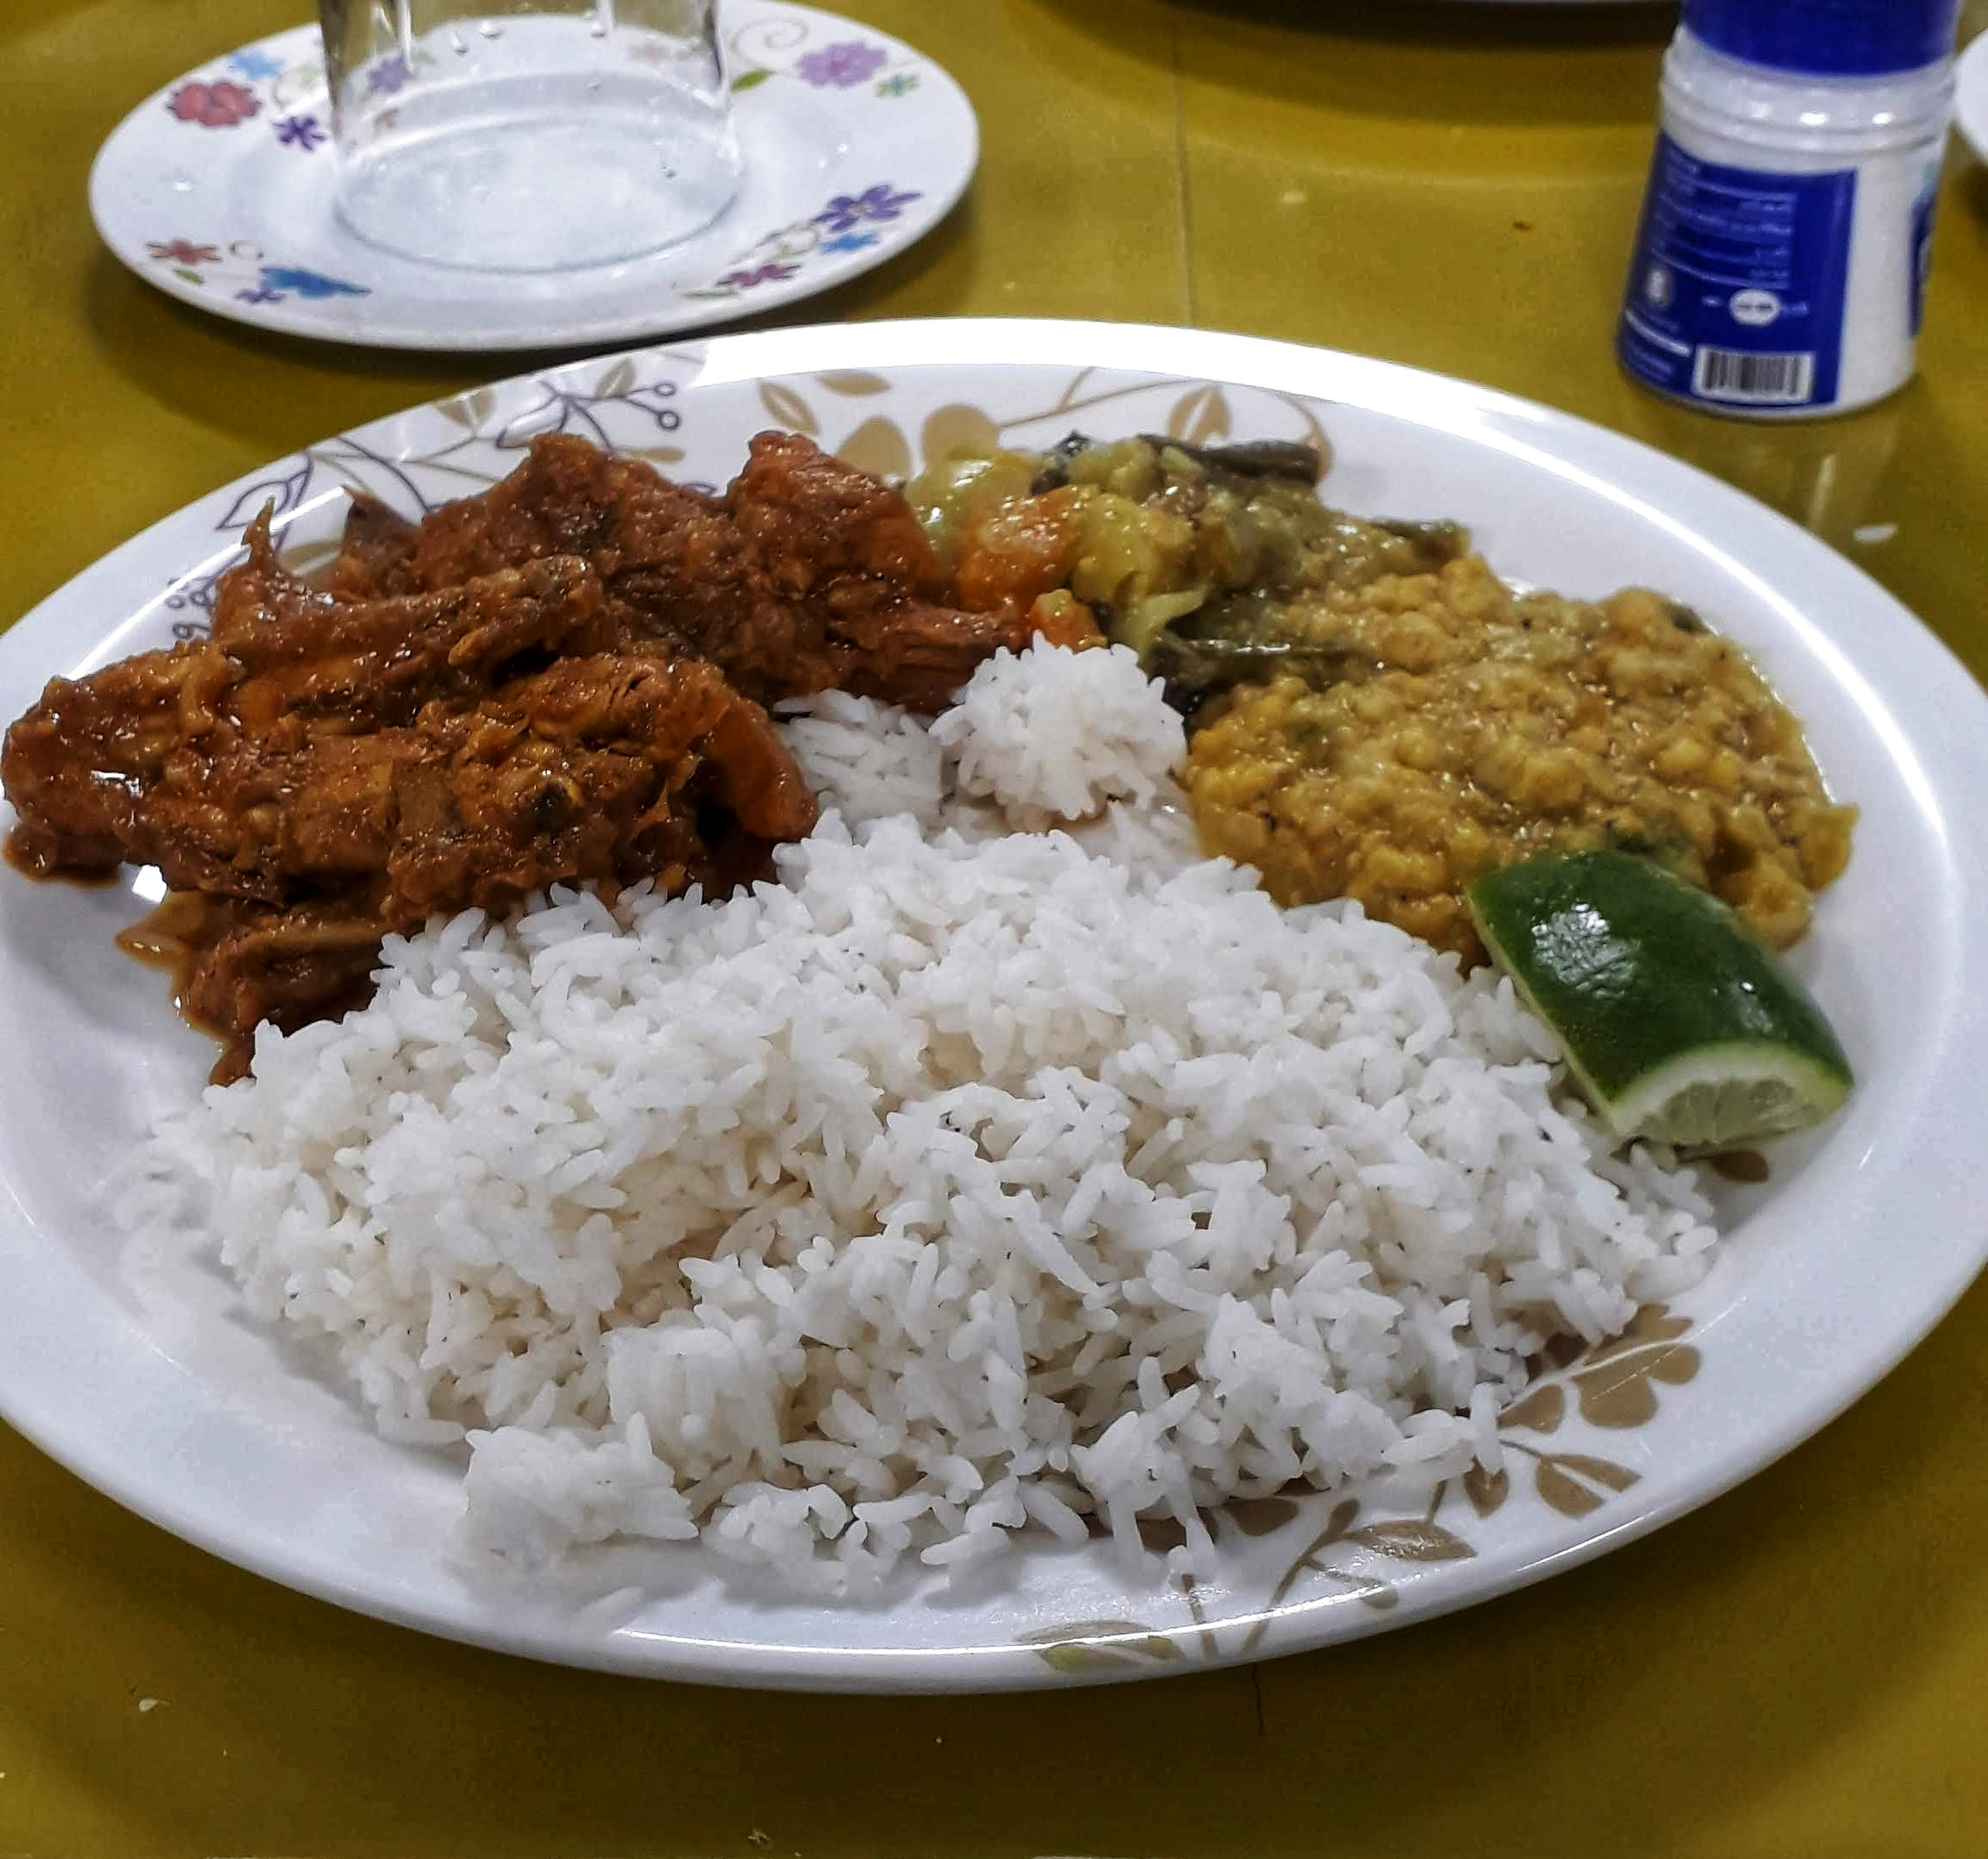
\includegraphics[width=4.6cm]{figures/context/meal_platter.jpg}};
\node[flnote,text width=4.6cm] at (2.35,-2.4) {可见食物与外观提供视觉线索\\实际重量和营养需要估计};

\node[fltrain,anchor=north west,text width=8.7cm,align=left,inner sep=8pt] (caption) at (6.0,2.9)
 {\textbf{\color{FLBlue}任务一 · 英文描述示例}\\[4pt]
 A plate of white rice with several side dishes.};
\node[flaccent,anchor=north west,text width=8.7cm,align=left,inner sep=8pt] (record) at (6.0,1.15)
 {\textbf{\color{FLBlue}任务二 · JSON 字段示例}\\[4pt]
 {\ttfamily\fontsize{8.5}{10.5}\selectfont
 \{\\
 \hspace*{1em}"items": [\{"name": "rice", "weight\_g": null\}],\\
 \hspace*{1em}"total\_weight\_g": null,\\
 \hspace*{1em}"total\_calories\_kcal": null,\\
 \hspace*{1em}"protein\_g": null,\\
 \hspace*{1em}"fat\_g": null,\\
 \hspace*{1em}"carbohydrate\_g": null\\
 \}}\\[4pt]
 {\fontsize{8}{10}\selectfont\color{FLMid}仅列一项食材；null 表示待估，实际输出须为数值。}};
\draw[flarrow] (4.72,.95) -- ++(.55,0) |- (caption.west);
\draw[flarrow] (4.72,-.6) -- ++(.55,0) |- (record.west);

\draw[FLLine,dashed] (0,-3.65)--(15.25,-3.65);
\node[fllabel,anchor=west] at (0,-4.0) {训练衔接：描述模型如何成为 Hybrid};
\node[flnode,text width=3.7cm,minimum height=.85cm] (source) at (2.05,-4.85)
 {任务一训练好的模型 A\\图像描述能力};
\node[flaccent,text width=4.65cm,minimum height=.85cm] (transfer) at (7.6,-4.85)
 {迁移视觉编码器与 GRU\\新增重量、营养回归头};
\node[fltrain,text width=3.7cm,minimum height=.85cm] (hybrid) at (13.15,-4.85)
 {任务二数据联合训练\\得到 Hybrid 模型};
\draw[flarrow] (source.east)--(transfer.west);
\draw[flarrow] (transfer.east)--(hybrid.west);
\end{tikzpicture}


\caption{餐食输入、两类输出示例与 Hybrid 的训练衔接。文字和字段为人工示意，非模型预测；null 为待估占位，实际预测需填入数值。}
\label{fig:meal-evidence}
\vspace{2pt}
{\scriptsize\color{FLMid}照片：Sm faysal，\href{https://commons.wikimedia.org/wiki/File:Plain_rice_chicken_vegetables_lintel_\%26_lemon_lunch_platter_from_Bangladesh.jpg}{Wikimedia Commons}，\href{https://creativecommons.org/licenses/by-sa/4.0/}{CC BY-SA 4.0}；仅等比例缩放。}
\end{figure}

\subsection{相关研究基础与关键困难}
\textbf{从全局概括到局部辨识。}经典图像描述方法建立了视觉编码与语言生成的联系，空间注意力进一步使模型在生成不同词语时读取不同区域\cite{vinyals2015show,xu2015attend}。Food-500 Cap 将评价落到菜品、可见食材和属性等细粒度内容\cite{ma2023food}。但烹饪改变外观、配料占比小和相互遮挡，使主要菜品正确而局部细节遗漏成为需要单独分析的问题。本项目据此比较全局与网格表示，并用消融实验辅助解释空间信息的作用。

\textbf{从食材语义到定量记录。}Inverse Cooking 研究图像中的食材预测及其与语言生成的联系，Nutrition5k 则以物理测量和营养标注支持份量与营养估计\cite{salvador2019inverse,thames2021nutrition}。二者提示，回答“有什么”与“有多少”需要不同监督。单张 RGB 图像缺少可靠尺度，投影面积也不能确定厚度、密度与遮挡份量；油脂等隐含成分进一步增加误差。本项目将食材生成与数值回归结合，分别评价识别错误与定量偏差，不将视觉上合理的输出视为真实测量。

\textbf{从文本相似到图像事实。}同一餐食可以有多种正确描述，而 Food-500 Cap 每图只有一条参考，词语重合指标对合理改写的覆盖有限。生成模型还可能依据常见搭配补出图中缺乏证据的食材。CLIPScore、FLEUR 等研究提供了直接结合图像评价描述的思路\cite{hessel2021clipscore,lee2024fleur}，但自动评价仍需检查其判断偏差。因此，本项目同时分析传统指标、视觉条件 Judge 与人工评分，检验指标提升是否伴随事实质量改善。各研究路线的详细比较见第~\ref{sec:related-work}~节。

\subsection{研究问题与任务设置}
\textbf{任务一：空间信息是否有助于食物细节描述？}在 Food-500 Cap 上自主实现两种课程指定结构：模型 A 采用 ResNet-18 全局表示与 GRU，模型 B 采用 ResNet-18 网格表示与 Transformer 编解码器。统一图文划分、词表规则和贪心解码，报告 BLEU-4、METEOR、ROUGE-L、CIDEr-D。A/B 比较反映两条路线的整体差异；另设保留 B 编解码配置、仅压缩视觉输入的 B-global，辅助分析空间信息贡献，并检查同图输出中的食材遗漏与属性误识别。

\textbf{任务二：描述模型的迁移与预训练模型的领域适配各有何收益？}采用教学云平台数据，保留训练、验证、测试的原始划分，分别为 2\,338、414、506 条。自主路线将 A 的视觉与序列参数迁移到 Hybrid，生成食材名称及对应重量，并独立回归整餐总重量、热量、蛋白质、脂肪和碳水化合物，组装为统一 JSON。通过“仅视觉迁移”与“视觉加 GRU 迁移”比较序列参数复用的作用。预训练路线拟采用 Qwen3-VL-4B-Instruct 与 LoRA，在相同基础版本、输入和解码条件下比较适配前后，再与 Hybrid 对照\cite{hu2022lora}。两条路线均报告任务一文本指标、食材名称 F1 和数值 MSE，补充逐字段误差及 Schema 有效率；质量单位为 g，热量单位为 kcal。

\textbf{选做实验：奖励优化的收益是否与视觉事实一致？}本组选择 SCST 与 Judge 两个方向，均纳入交付。SCST 从选定的 A 交叉熵权重出发，以 CIDEr-D 为奖励，并与原始交叉熵版本及等步数继续交叉熵版本比较\cite{rennie2017scst}。Judge 对匿名描述的语义正确性、内容覆盖、幻觉和流畅度评分，再与双人独立评分及传统指标对照。实验检验收益及其局限，不预设奖励提升必然减少幻觉。

\subsection{预期贡献与研究边界}
本项目的设计特色体现在三个可检验的方面：一是将描述模型的视觉与序列能力迁移到结构化膳食任务，通过迁移对照检验复用价值；二是在完整食材名称的生成边界对齐重量预测，结合独立整餐回归形成语义与数值联合输出，并分解其错误来源；三是将序列奖励优化与图像事实评价结合，分析自动指标和人工判断之间的一致与分歧。上述内容属于面向课程任务的结构设计与实验探索，效果由后续实验验证，具体实现见第~\ref{sec:technical-plan}~节。

食堂是应用动机，当前结论限定于指定数据与划分，尚不能据此宣称对校园真实餐食的泛化效果。Food500 图文需经可追溯映射、哈希与重复组核验后固定清单；词表、数值统计和奖励统计仅由训练集拟合，验证集用于选模。测试前冻结模型与评价协议，推理只读取 RGB、必要的样本标识和固定指令；评价保留缺失、截断及解析失败，以全部目标样本为分母。正式训练效果与 GPU 资源数据均有待实测。

